% !TeX root = ../../Skript.tex
\cohead{\Large\textbf{Einführung Exponentialfunktionen}}
\fakesubsection{Einführung Exponentialfunktionen}
Die Anzahl der Bakterien in einer Petrischale verdoppelt sich jede Stunde (bis die komplette Schale mit Bakterien bedeckt ist). Zu Beginn sind 10 Bakterien auf der Schale. Vervollständige die Tabelle:

\resizebox{\textwidth}{!}{\begin{tabular}{c||c|c|c|c|c|c|c}
		\(x\)&0&1&2&3&4&5&6\\
		\hline
		\multirow{2}{1cm}{\(f(x)\)}&10&20&\textcolor{loes}{40}&\textcolor{loes}{80}&\textcolor{loes}{160}&\textcolor{loes}{320}&\textcolor{loes}{640}\\
		&\textcolor{loes}{\(10\cdot2^0\)}&\textcolor{loes}{\(10\cdot2^1\)}&\textcolor{loes}{\(10\cdot2^2\)}&\textcolor{loes}{\(10\cdot2^3\)}&\textcolor{loes}{\(10\cdot2^4\)}&\textcolor{loes}{\(10\cdot2^5\)}&\textcolor{loes}{\(10\cdot2^6\)}
\end{tabular}}

\bigskip

\begin{minipage}{\textwidth}
\adjustbox{valign=t}{\begin{minipage}{0.5\textwidth}\raggedright
	\scalebox{2}{\(f(x)= \textcolor{loes}{10\cdot 2^x}\)}

    \bigskip

	Wie viele Bakterien sind nach 20h und nach 100h vorhanden?

	\textcolor{loes}{Da \(x\) die Zeit in Stunden angibt, setzt man einfach die angegebenen Werte ein:}
	\begin{align*}
		\textcolor{loes}{f(20)}&\textcolor{loes}{=10\cdot 2^{20}=10.485.760}\\
		\textcolor{loes}{f(100)}&\textcolor{loes}{=10\cdot 2^{100}\approx 1,27\cdot 10^{31}}
	\end{align*}
	Nach wie vielen Stunden waren 8000 Bakterien vorhanden?

	\textcolor{loes}{\(f(x)\) gibt die Anzahl an Bakterien nach \(x\) Stunden an. Wir setzen also gleich:}
	\begin{align*}
		\textcolor{loes}{f(x)}&\textcolor{loes}{=8000}\\
		\textcolor{loes}{10\cdot 2^x}&\textcolor{loes}{=8000\,\vert\,:10}\\
		\textcolor{loes}{2^x}&\textcolor{loes}{=800\,\vert\,\log_2}\\
		\textcolor{loes}{\Rightarrow x}&\textcolor{loes}{=\log_2(800)\approx 9,64}
	\end{align*}
	\textcolor{loes}{Der Logarithmus erfüllt für Exponentialfunktionen die gleiche Funktion, die die verschiedenen Wurzeln für \(x^2,\ x^3,\) usw. erfüllen.}
\end{minipage}}%
\adjustbox{valign=t, padding =2ex 0ex 0ex 0ex}{\begin{minipage}{0.5\textwidth-2ex}\centering
	\iftoggle{ausfuellen}{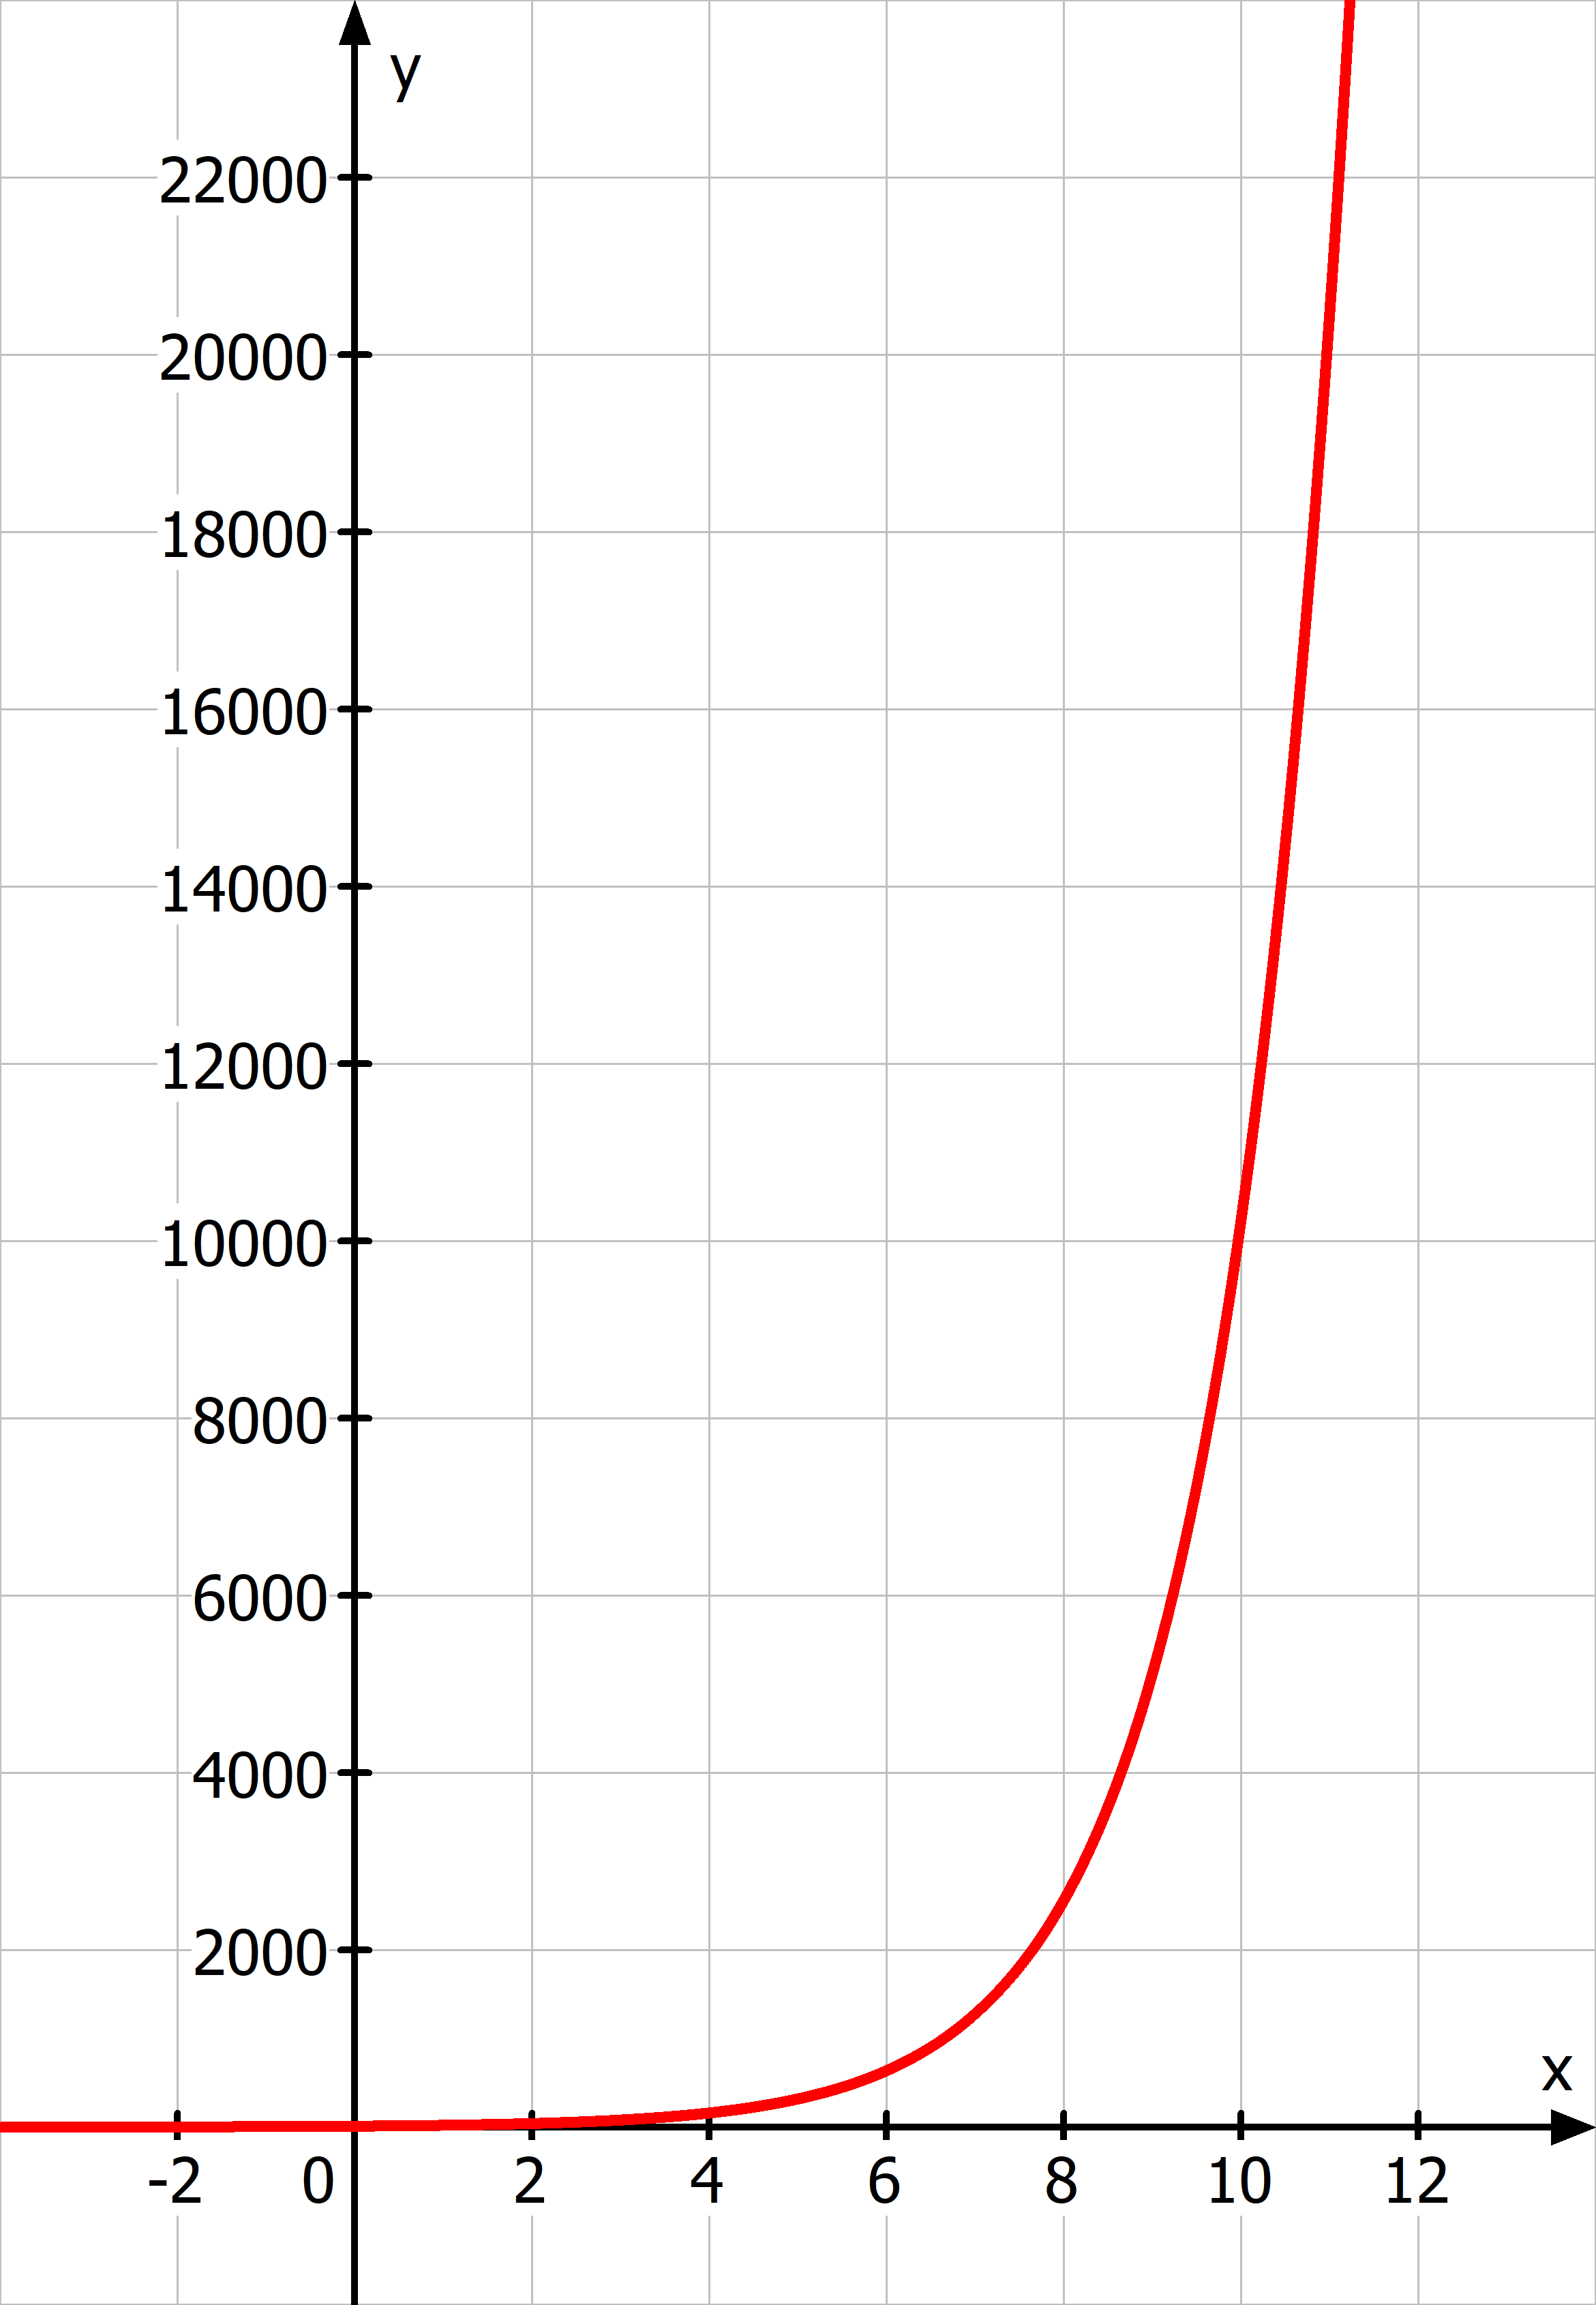
\includegraphics[width=\textwidth]{\eFkt/pics/bakterien.png}}{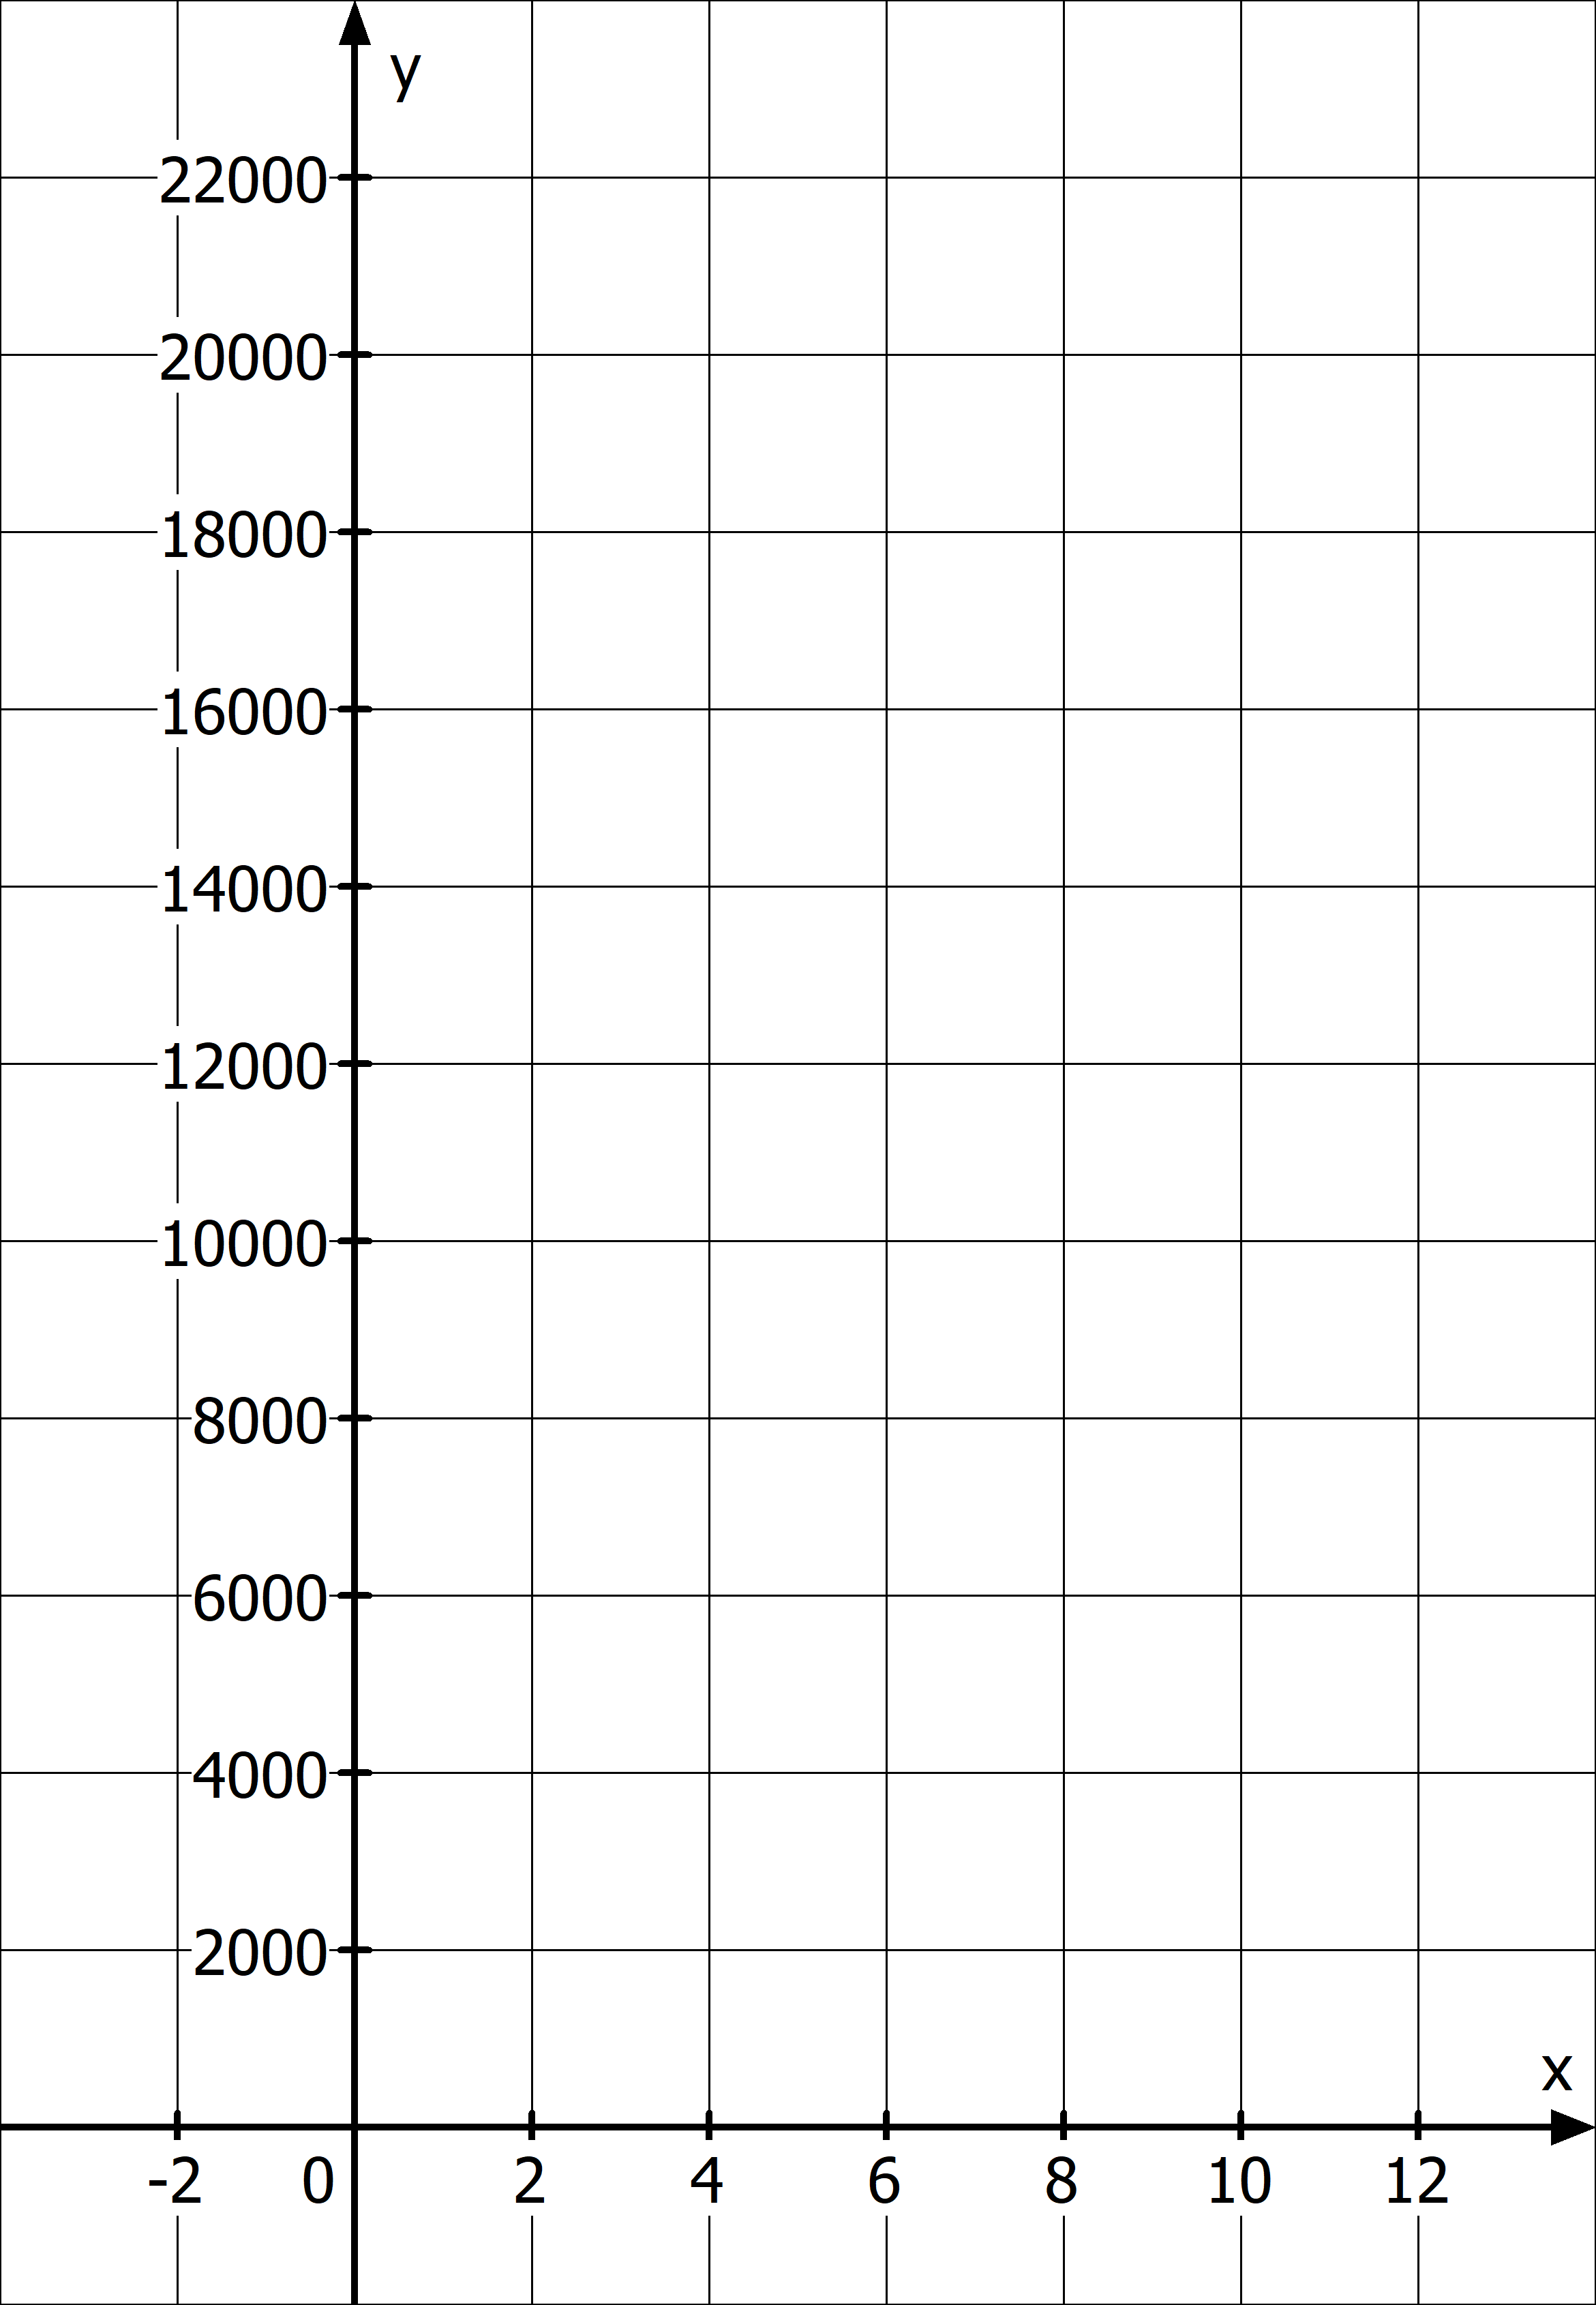
\includegraphics[width=\textwidth]{\eFkt/pics/bakterien_empty.png}}
\end{minipage}}%
\end{minipage}
Exponentialfunktionen wie \(2^x\) wachsen sehr schnell. Überlegen wir uns zur Illustration wie lange es dauern würde bis die komplette Erde (\(m_{Erde}=6\cdot 10^{24}kg\)) aus Bakterien bestehen würde, falls sie sich unbegrenzt vermehren könnten. 1.000.000.000.000.000 Bakterien wiegen 1g.
\begin{align*}
	\textcolor{loes}{f(x)}&\textcolor{loes}{=6\cdot 10^42}\\
	\textcolor{loes}{10\cdot 2^x}&\textcolor{loes}{=6\cdot 10^42\,\vert\,:10}\\
	\textcolor{loes}{2^x}&\textcolor{loes}{=6\cdot 10^41\,\vert\,\log_2}\\
	\textcolor{loes}{\Rightarrow x}&\textcolor{loes}{=\log_2\left( 6\cdot 10^41\right) \approx 138,8}
\end{align*}
\textcolor{loes}{Könnten sich die Bakterien unbegrenzt vermehren, würde es also lediglich \(139h=5,8d\), also nicht ganz 6 Tage, dauern bis die komplette Erde nur aus Bakterien bestehen würde.}
\newpage
%%%%%%%%%%%%%%%%%%%%%%%%%%%%%%%%%%%%%%%%%%%%%%%%%%%%%%%%%%%%%%%%%%%%%%%%%%%%%%%%%%%%%%%%%%%%%%%%%%%%%%
Das Isotop \(^{207}\)Ra hat eine Halbwertszeit von ca. 1s, d.h. dass innerhalb einer Sekunde die Hälfte des radioaktiven Materials in andere Elemente zerfallen ist. Zu Beginn sind 8g Radium vorhanden. Vervollständige die Tabelle:\\
\resizebox{\textwidth}{!}{\begin{tabular}{c||c|c|c|c|c|c|c}
		\(x\)&0&1&2&3&4&5&6\\
		\hline
		\multirow{2}{1cm}{\(f(x)\)}
		&8
		&4
		&\textcolor{loes}{2}
		&\textcolor{loes}{1}
		&\textcolor{loes}{\(\frac{1}{2}\)}
		&\textcolor{loes}{\(\frac{1}{4}\)}
		&\textcolor{loes}{\(\frac{1}{8}\)}\\
		&\textcolor{loes}{\(8\cdot\left(\frac{1}{2}\right)^0\)}
		&\textcolor{loes}{\(8\cdot\left(\frac{1}{2}\right)^1\)}
		&\textcolor{loes}{\(8\cdot\left(\frac{1}{2}\right)^2\)}
		&\textcolor{loes}{\(8\cdot\left(\frac{1}{2}\right)^3\)}
		&\textcolor{loes}{\(8\cdot\left(\frac{1}{2}\right)^4\)}
		&\textcolor{loes}{\(8\cdot\left(\frac{1}{2}\right)^5\)}
		&\textcolor{loes}{\(8\cdot\left(\frac{1}{2}\right)^6\)}
\end{tabular}}

\bigskip

\begin{minipage}{\textwidth}
\adjustbox{valign=t}{\begin{minipage}{0.4\textwidth}\raggedright
	\scalebox{2}{\(f(x)= \textcolor{loes}{8\cdot \left(\frac{1}{2}\right)^x}\)}

    \bigskip

	Wie viel \(g\) Radium sind nach 10s noch vorhanden, wie viel nach 1min?

	\textcolor{loes}{Da \(x\) die Zeit in Sekunden angibt, setzt man einfach die angegebenen Werte ein:}

    \adjustbox{valign=t}{\begin{minipage}{\textwidth}
	\begin{align*}
		\textcolor{loes}{f(10)}&\textcolor{loes}{\;=8\cdot \left(\frac{1}{2}\right)^{10}=\frac{1}{128}\approx 0,00781}\\
		\textcolor{loes}{f(60)}&\textcolor{loes}{\;=8\cdot \left(\frac{1}{2}\right)^{60}\approx 6,94\cdot10^{-18}}
	\end{align*}%
    \end{minipage}}%
\end{minipage}}%
\adjustbox{valign=t, padding =2ex 0ex 0ex 0ex}{\begin{minipage}{0.6\textwidth-2ex}\centering
	\iftoggle{ausfuellen}{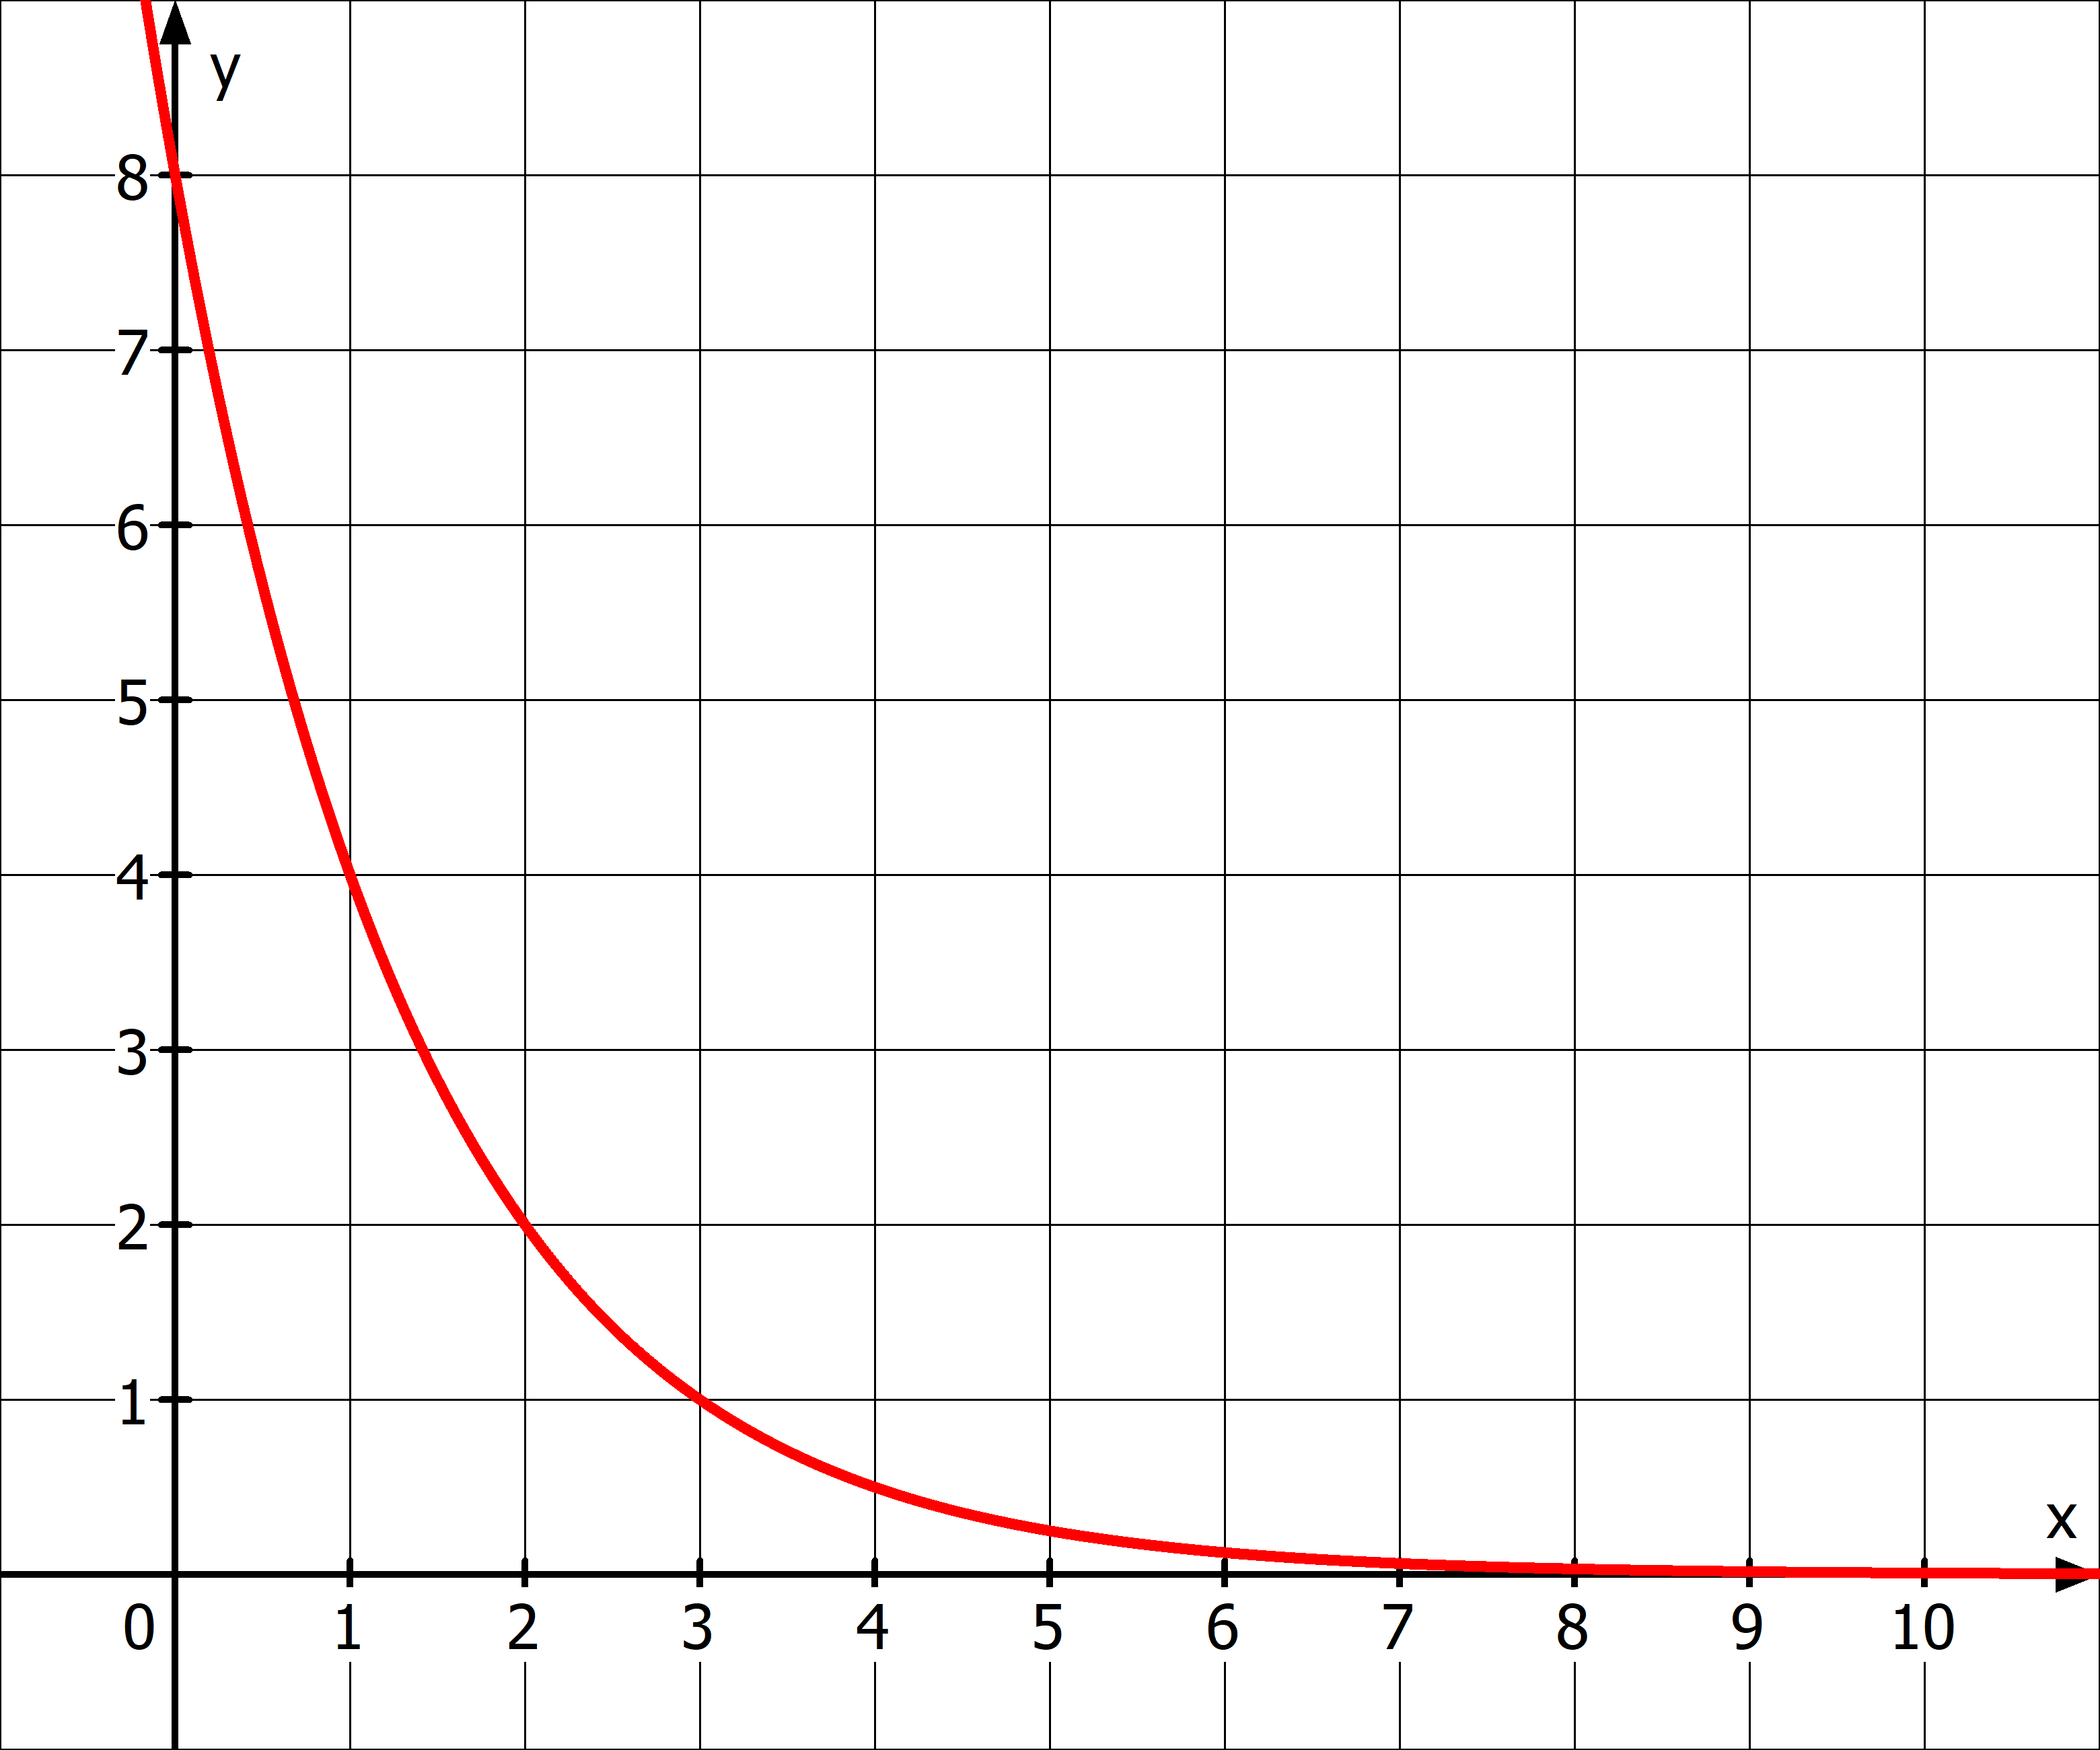
\includegraphics[width=\textwidth]{\eFkt/pics/radium.png}}{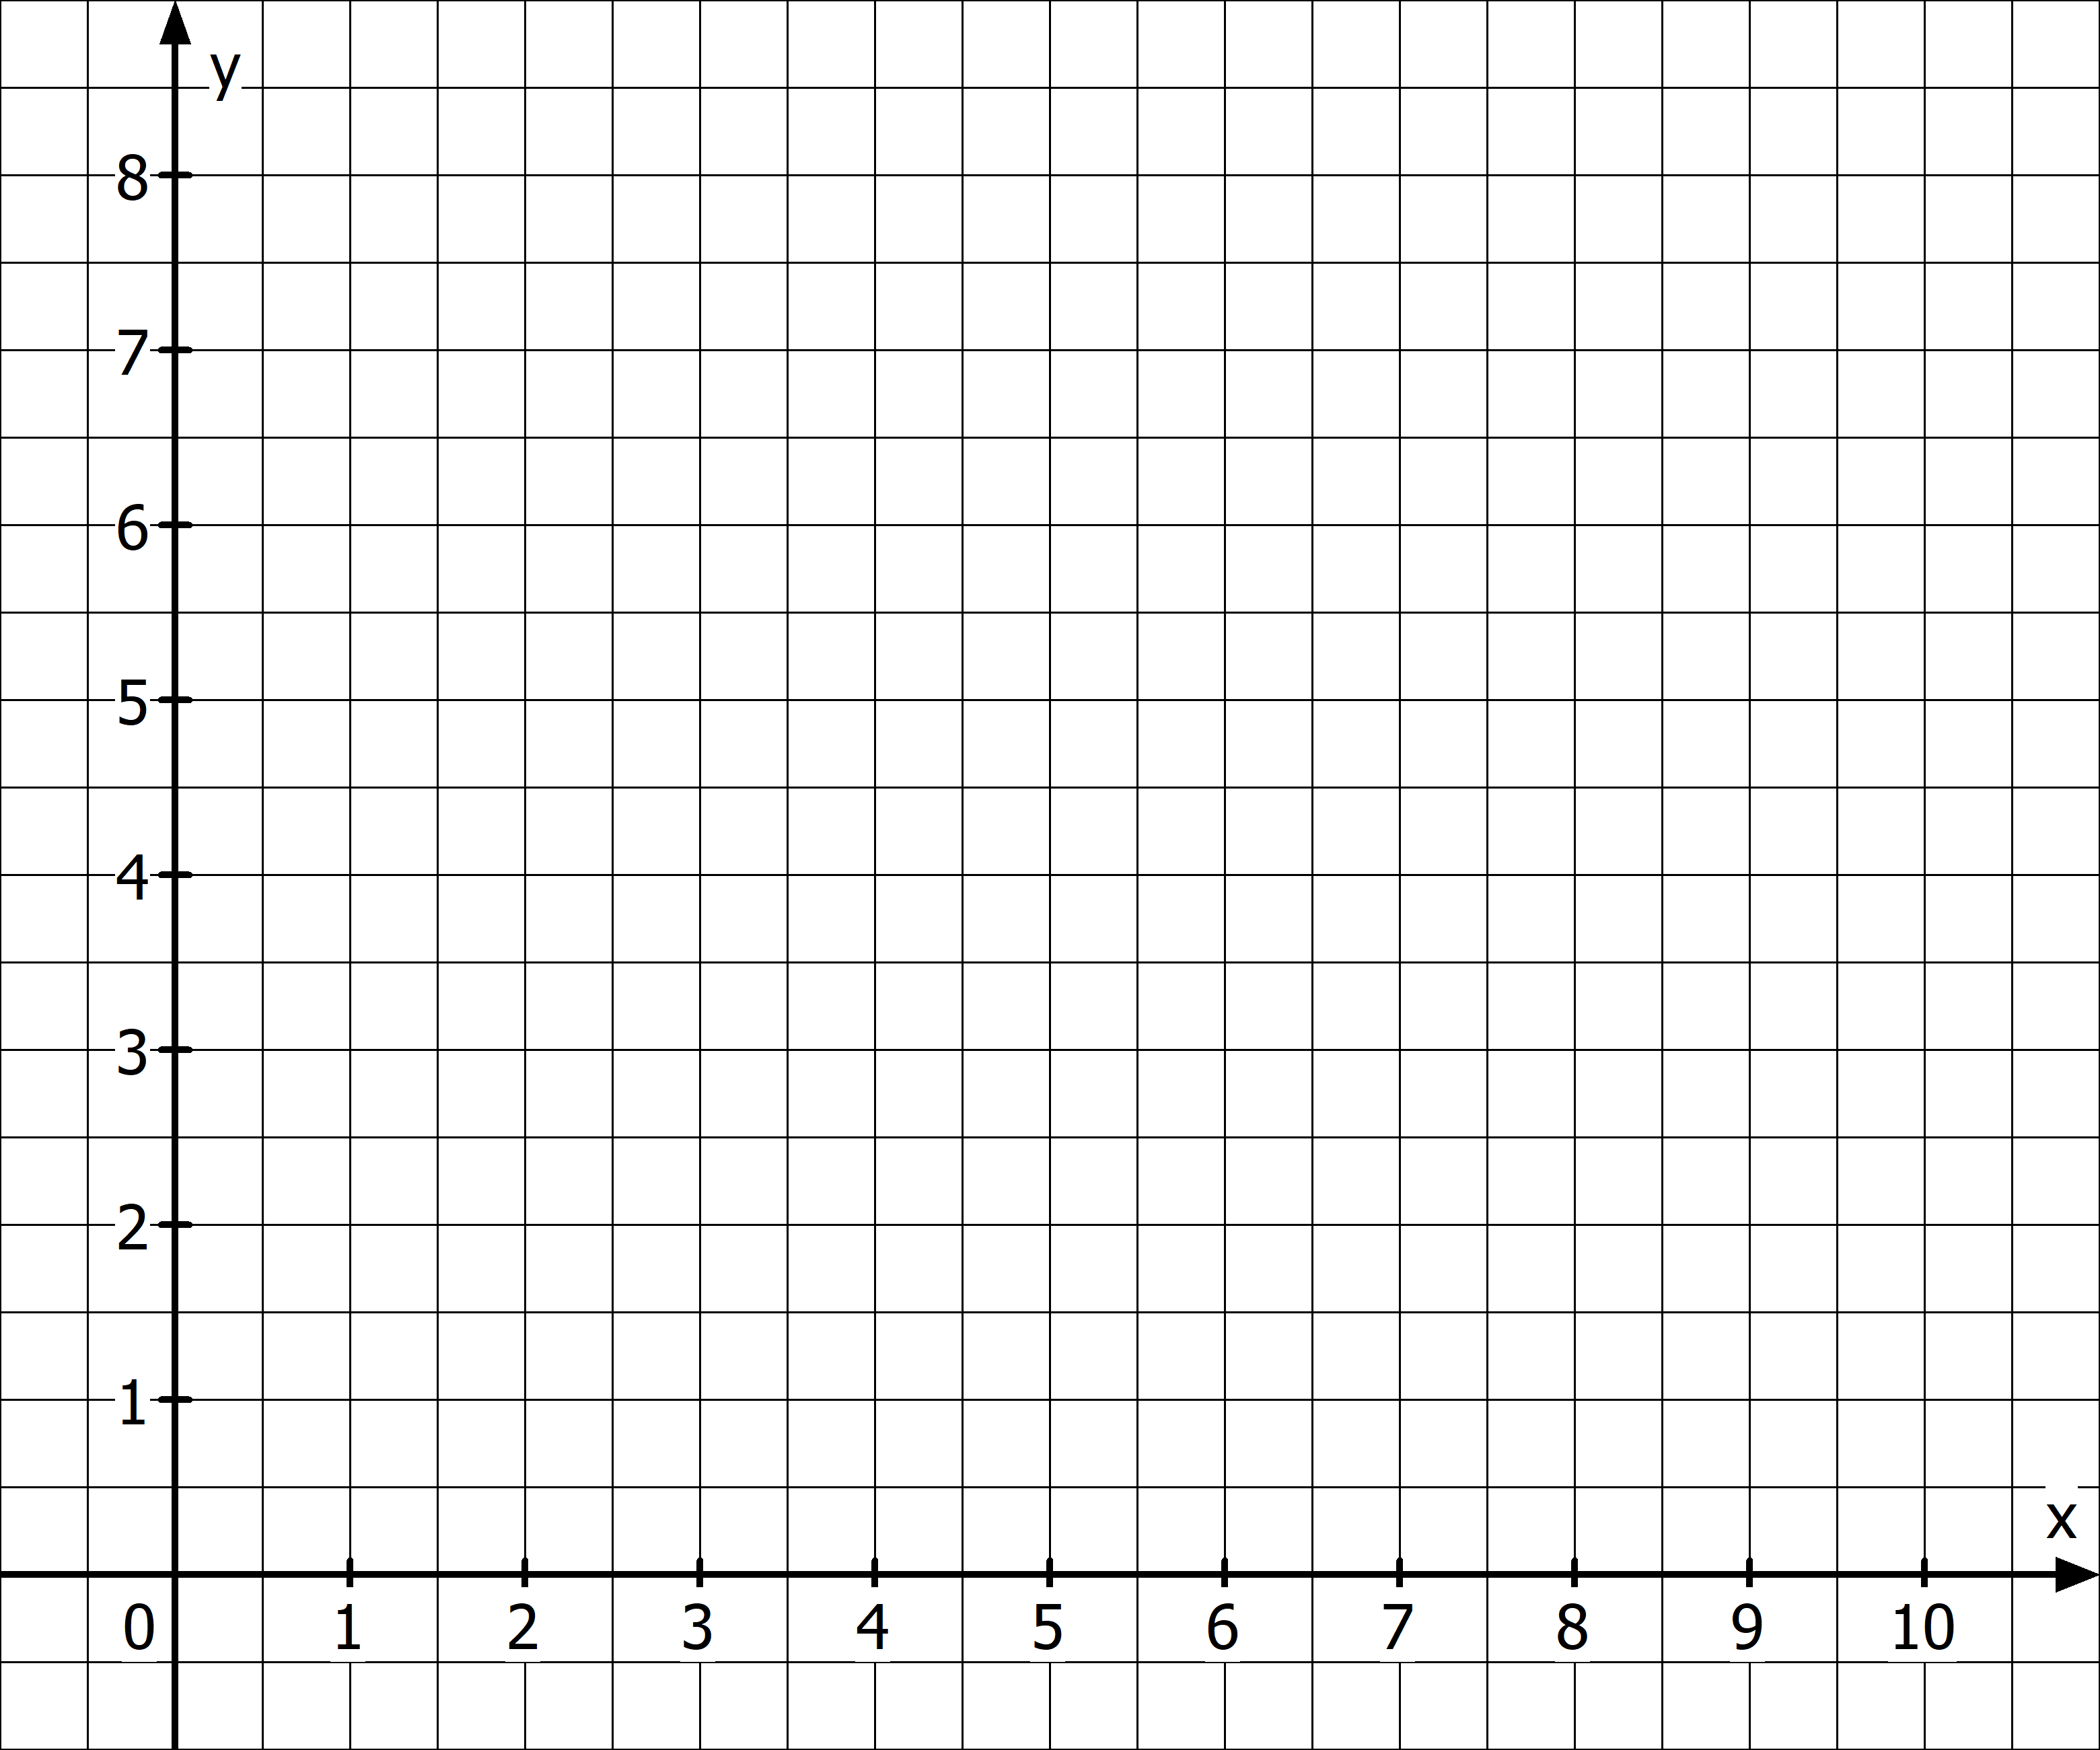
\includegraphics[width=\textwidth]{\eFkt/pics/radium_empty.png}}
\end{minipage}}%
\end{minipage}

\medskip

Nach wie vielen Sekunden waren noch 0,3g Radium vorhanden?\\
\textcolor{loes}{\(f(x)\) gibt die Masse des Radiums in \(g\) nach \(x\) Sekunden an. Wir setzen also gleich:}
\begin{align*}
	\textcolor{loes}{f(x)}&\textcolor{loes}{=0,3}\\
	\textcolor{loes}{8\cdot \left(\frac{1}{2}\right)^x}&\textcolor{loes}{=0,3\,\vert\,:8}\\
	\textcolor{loes}{\left(\frac{1}{2}\right)^x}&\textcolor{loes}{=\frac{3}{80}\,\vert\,\log_{\frac{1}{2}}}\\
	\textcolor{loes}{\Rightarrow x}&\textcolor{loes}{=\log_{\frac{1}{2}}\left(\frac{3}{80}\right) \approx 4,74}
\end{align*}
Wie lange würde es dauern bis die Masse des Radiums die eines Bakteriums entspricht?
\begin{align*}
	\textcolor{loes}{f(x)}&\textcolor{loes}{=10^{-15}}\\
	\textcolor{loes}{8\cdot \left(\frac{1}{2}\right)^x}&\textcolor{loes}{=10^{-15}\,\vert\,:8}\\
	\textcolor{loes}{\left(\frac{1}{2}\right)^x}&\textcolor{loes}{=1,25\cdot 10^{-16}\,\vert\,\log_{\frac{1}{2}}}\\
	\textcolor{loes}{\Rightarrow x}&\textcolor{loes}{=\log_{\frac{1}{2}}\left(1,25\cdot 10^{-16}\right) \approx 52,8}
\end{align*}
\textcolor{loes}{Es dauert also nicht mal ganz eine Minute bis das Radium fast verschwunden ist.}